

\begin{center}
\thispagestyle{empty}
%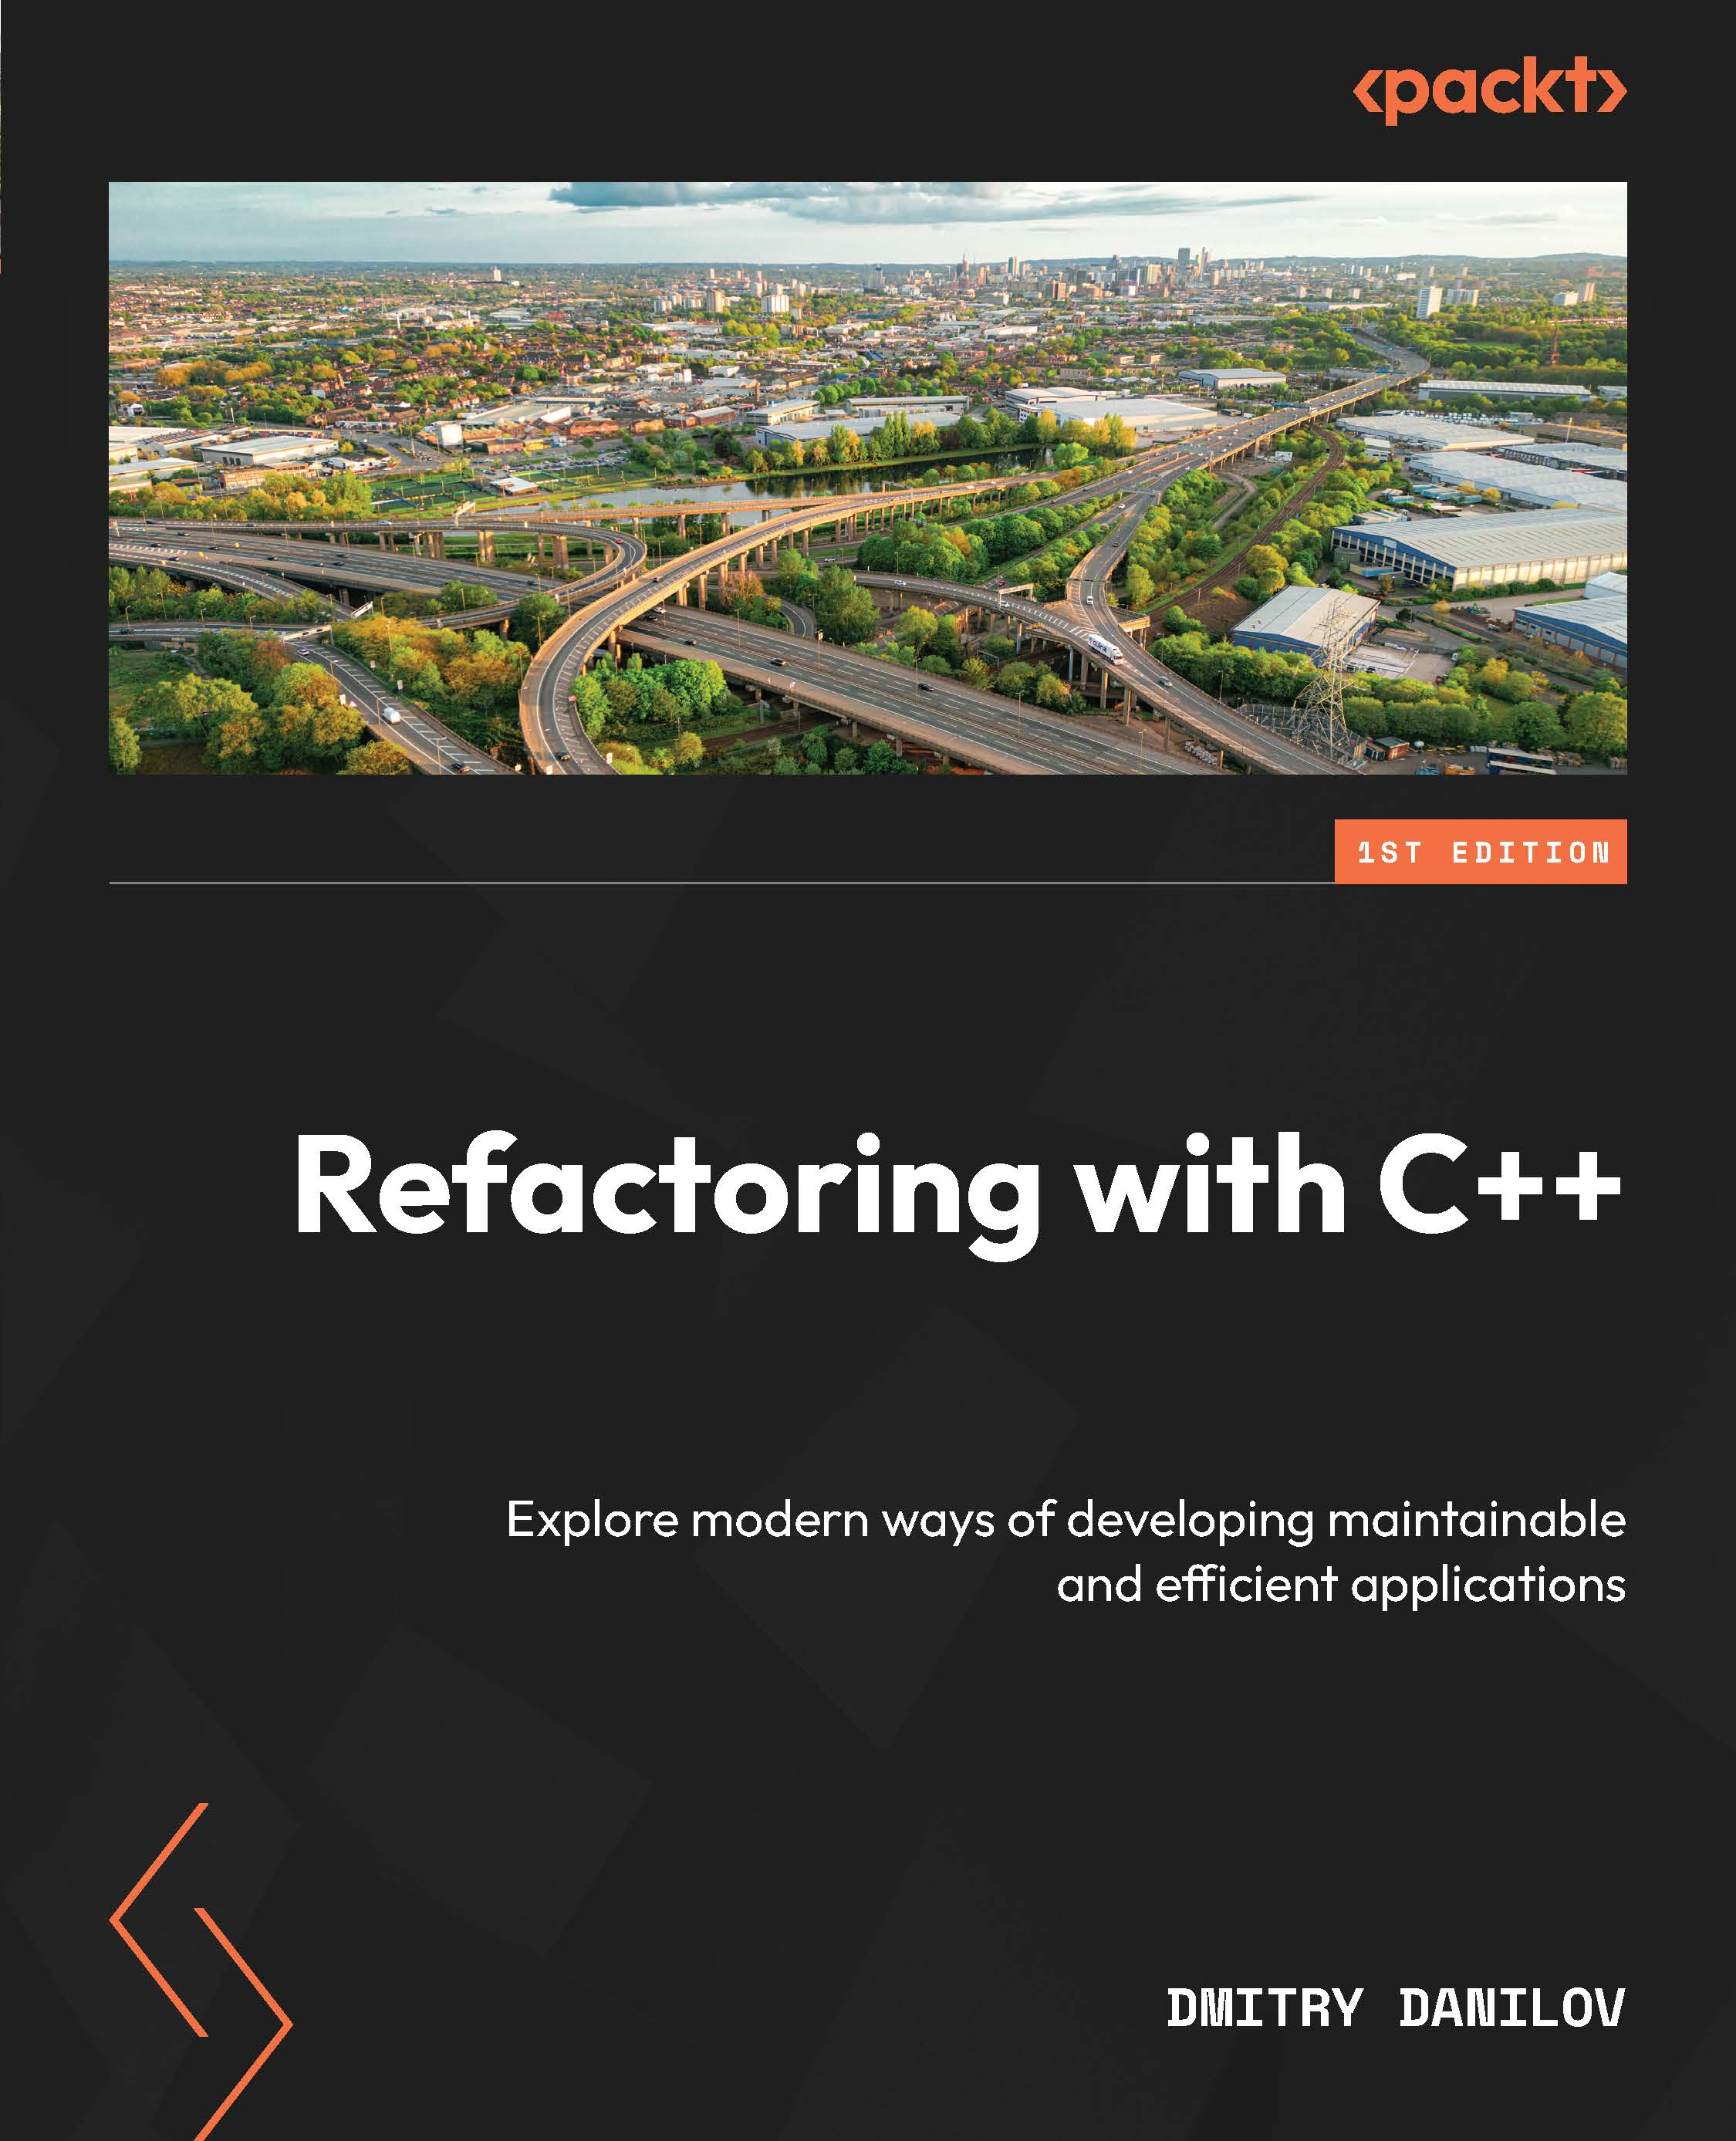
\includegraphics[width=\textwidth,height=\textheight,keepaspectratio]{cover.png}
\begin{tikzpicture}[remember picture, overlay, inner sep=0pt]
\node at (current page.center)
{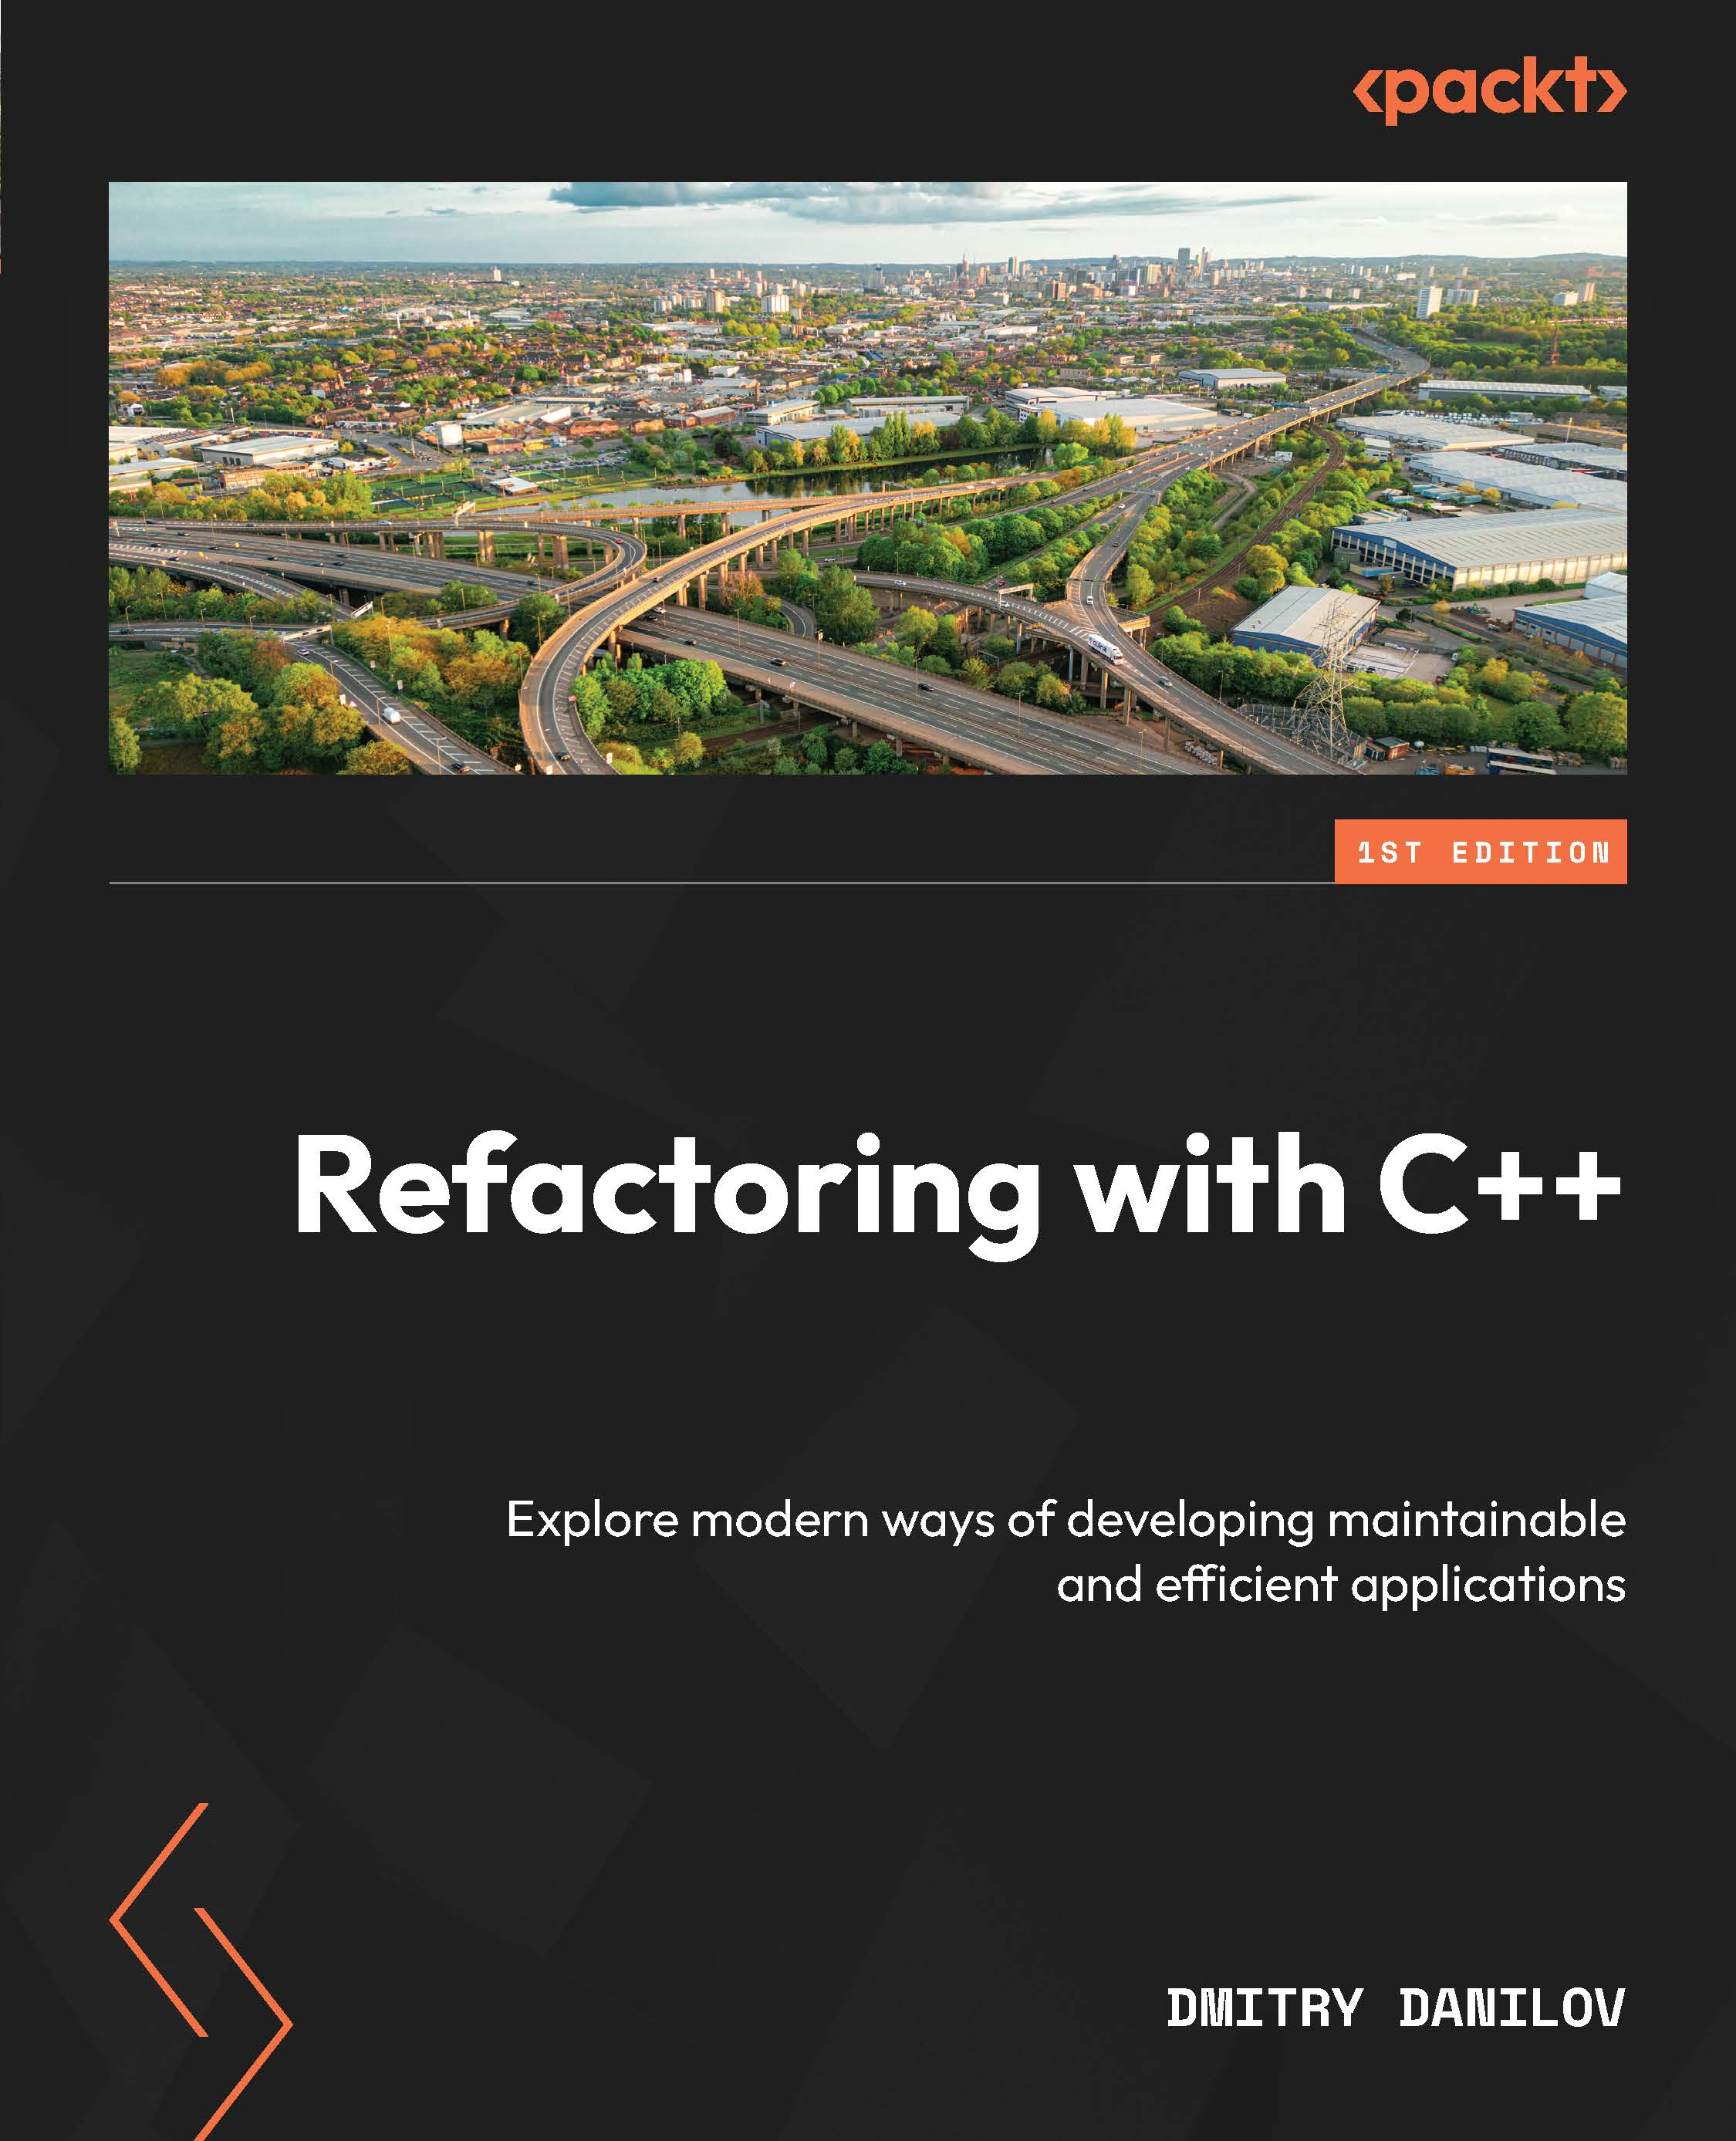
\includegraphics[width=\paperwidth, keepaspectratio=false]{cover.png}};
\end{tikzpicture}
\newpage
\thispagestyle{empty}
\huge
\textbf{以重构为名,开发现代高效C++应用}
\\[9pt]
\normalsize
作者: Dmitry Danilov
\\[8pt]
\normalsize
译者:\href{https://github.com/xiaoweiChen/Refactoring-with-Cpp}{陈晓伟}
\\[8pt]
\end{center}

\newpage

\begin{comment}
\end{comment}

\pagestyle{empty}
\tableofcontents
\newpage

\setsecnumdepth{section}

\myChapter{关于作者}{}{content/about-the-author.tex}
\newpage

\myChapter{关于评审}{}{content/about-the-reviewer.tex}
\newpage

\myChapter{前言}{}{content/preface.tex}
\newpage

\myChapter{第1章}{C++编码标准}{content/chapter1/0.tex}
\mySubsection{1.1.}{好代码与坏代码}{content/chapter1/1.tex}
\mySubsection{1.2.}{编码标准}{content/chapter1/2.tex}
\mySubsection{1.3.}{可读性、效率、可维护性和可用性}{content/chapter1/3.tex}
\mySubsection{1.4.}{总结}{content/chapter1/4.tex}
\newpage

\myChapter{第2章}{主要软件开发原则}{content/chapter2/0.tex}
\mySubsection{2.1.}{SOLID}{content/chapter2/1.tex}
\mySubsection{2.2.}{KISS 原则}{content/chapter2/2.tex}
\mySubsection{2.3.}{副作用和不变性}{content/chapter2/3.tex}
\mySubsection{2.4.}{总结}{content/chapter2/4.tex}
\newpage

\myChapter{第3章}{错误代码的成因}{content/chapter3/0.tex}
\mySubsection{3.1.}{需要交付产品}{content/chapter3/1.tex}
\mySubsection{3.2.}{开发者的个人品味}{content/chapter3/2.tex}
\mySubsection{3.3.}{C++中同一问题的多种解法}{content/chapter3/3.tex}
\mySubsection{3.4.}{缺乏对现代 C++ 的了解}{content/chapter3/4.tex}
\mySubsection{3.5.}{指针使用不足}{content/chapter3/5.tex}
\mySubsection{3.6.}{总结}{content/chapter3/6.tex}
\newpage

\myChapter{第4章}{确定重写的理想候选 --- 模式和反模式}{content/chapter4/0.tex}
\mySubsection{4.1.}{什么样的代码值得重写?}{content/chapter4/1.tex}
\mySubsection{4.2.}{异味代码}{content/chapter4/2.tex}
\mySubsection{4.3.}{反模式}{content/chapter4/3.tex}
\mySubsection{4.4.}{遗留代码}{content/chapter4/4.tex}
\mySubsection{4.5.}{总结}{content/chapter4/5.tex}
\newpage

\myChapter{第5章}{命名的意义}{content/chapter5/0.tex}
\mySubsection{5.1.}{一般性命名原则}{content/chapter5/1.tex}
\mySubsection{5.2.}{探索主流 C++ 编码约定 --- Google、 LLVM 和 Mozilla}{content/chapter5/2.tex}
\mySubsection{5.3.}{总结}{content/chapter5/3.tex}
\newpage

\myChapter{第6章}{使用静态类型}{content/chapter6/0.tex}
\mySubsection{6.1.}{使用 Chrono 来计算时间长度}{content/chapter6/1.tex}
\mySubsection{6.2.}{使用 not\_null 和 std::optional 提高指针安全性}{content/chapter6/2.tex}
\mySubsection{6.3.}{使用枚举类和范围枚举进行强类型}{content/chapter6/3.tex}
\mySubsection{6.4.}{使用标准库的类型实用程序}{content/chapter6/4.tex}
\mySubsection{6.5.}{避免高级类型使用中的坑}{content/chapter6/5.tex}
\mySubsection{6.6.}{总结}{content/chapter6/6.tex}
\newpage

\myChapter{第7章}{C++中的类、对象和面向对象}{content/chapter7/0.tex}
\mySubsection{7.1.}{适合类的情景}{content/chapter7/1.tex}
\mySubsection{7.2.}{C++ 中的继承}{content/chapter7/2.tex}
\mySubsection{7.3.}{模板和泛型编程}{content/chapter7/3.tex}
\mySubsection{7.4.}{实例化模板}{content/chapter7/4.tex}
\mySubsection{7.5.}{模板使用示例}{content/chapter7/5.tex}
\mySubsection{7.6.}{总结}{content/chapter7/6.tex}
\newpage

\myChapter{第8章}{设计和开发 C++ API}{content/chapter8/0.tex}
\mySubsection{8.1.}{API 简约设计原则}{content/chapter8/1.tex}
\mySubsection{8.2.}{实现极简主义的技巧}{content/chapter8/2.tex}
\mySubsection{8.3.}{API 简约设计示例}{content/chapter8/3.tex}
\mySubsection{8.4.}{常见的坑及躲避方法}{content/chapter8/4.tex}
\mySubsection{8.5.}{开发共享库的注意事项}{content/chapter8/5.tex}
\mySubsection{8.6.}{总结}{content/chapter8/6.tex}
\newpage

\myChapter{第9章}{代码格式和命名约定}{content/chapter9/0.tex}
\mySubsection{9.1.}{为什么代码格式化很重要?}{content/chapter9/1.tex}
\mySubsection{9.2.}{有助于遵守编码约定的现有工具概述}{content/chapter9/2.tex}
\mySubsection{9.3.}{配置Clang-Format --- 深入了解自定义格式规则}{content/chapter9/3.tex}
\mySubsection{9.4.}{将 Clang-Format 集成到构建系统中}{content/chapter9/4.tex}
\mySubsection{9.5.}{Clang-Format 报告示例}{content/chapter9/5.tex}
\mySubsection{9.6.}{扩展 CI 的代码格式检查}{content/chapter9/6.tex}
\mySubsection{9.7.}{各种编辑器均支持 Clang-Format}{content/chapter9/7.tex}
\mySubsection{9.8.}{检查名称样式}{content/chapter9/8.tex}
\mySubsection{9.9.}{将 Clang-Tidy 集成到构建系统中}{content/chapter9/9.tex}
\mySubsection{9.10.}{使用 Clang-Tidy 检查源代码名称样式}{content/chapter9/10.tex}
\mySubsection{9.11.}{自动修复命名问题}{content/chapter9/11.tex}
\mySubsection{9.12.}{示例项目}{content/chapter9/12.tex}
\mySubsection{9.13.}{支持 Clang-Tidy的各种编辑器}{content/chapter9/13.tex}
\mySubsection{9.14.}{总结}{content/chapter9/14.tex}
\newpage

\myChapter{第10章}{静态分析}{content/chapter10/0.tex}
\mySubsection{10.1.}{静态分析的本质}{content/chapter10/1.tex}
\mySubsection{10.2.}{强化 C++ 代码的编译器设置}{content/chapter10/2.tex}
\mySubsection{10.3.}{通过多个编译器进行静态分析}{content/chapter10/3.tex}
\mySubsection{10.4.}{使用 Clang-Tidy 探索静态分析}{content/chapter10/4.tex}
\mySubsection{10.5.}{静态分析工具概述 --- PVS-Studio、 SonarQube 等与 Clang-Tidy 的比较}{content/chapter10/5.tex}
\mySubsection{10.6.}{总结}{content/chapter10/6.tex}
\newpage

\myChapter{第11章}{动态分析}{content/chapter11/0.tex}
\mySubsection{11.1.}{基于编译器}{content/chapter11/1.tex}
\mySubsection{11.2.}{使用 Valgrind}{content/chapter11/2.tex}
\mySubsection{11.3.}{Valgrind 套件中的其他工具}{content/chapter11/3.tex}
\mySubsection{11.4.}{总结}{content/chapter11/4.tex}
\newpage

\myChapter{第12章}{测试}{content/chapter12/0.tex}
\mySubsection{12.1.}{测试驱动开发}{content/chapter12/1.tex}
\mySubsection{12.2.}{单元测试}{content/chapter12/2.tex}
\mySubsection{12.3.}{单元测试框架}{content/chapter12/3.tex}
\mySubsection{12.4.}{Google Test 和 Google Mock}{content/chapter12/4.tex}
\mySubsection{12.5.}{将 Google Test 集成到 C++ 项目中}{content/chapter12/5.tex}
\mySubsection{12.6.}{C++ 项目中使用 Google Test}{content/chapter12/6.tex}
\mySubsection{12.7.}{编写简单测试}{content/chapter12/7.tex}
\mySubsection{12.8.}{使用测试固件}{content/chapter12/8.tex}
\mySubsection{12.9.}{主要功能}{content/chapter12/9.tex}
\mySubsection{12.10.}{运行 Google Test 测试}{content/chapter12/10.tex}
\mySubsection{12.11.}{Google Test 的高级功能}{content/chapter12/11.tex}
\mySubsection{12.12.}{C++ 项目中使用 gMock}{content/chapter12/12.tex}
\mySubsection{12.13.}{使用 gMock 的示例}{content/chapter12/13.tex}
\mySubsection{12.14.}{其他值得注意的 C++ 单元测试框架}{content/chapter12/14.tex}
\mySubsection{12.15.}{单元测试的良好候选者}{content/chapter12/15.tex}
\mySubsection{12.16.}{软件开发中的 E2E 测试}{content/chapter12/16.tex}
\mySubsection{12.17.}{有利于 E2E 测试的情况}{content/chapter12/17.tex}
\mySubsection{12.18.}{自动测试覆盖率跟踪工具}{content/chapter12/18.tex}
\mySubsection{12.19.}{总结}{content/chapter12/19.tex}
\newpage

\myChapter{第13章}{管理第三方的现代方法}{content/chapter13/0.tex}
\mySubsection{13.1.}{链接和共享 V threads::ThreadsS 静态库概述}{content/chapter13/1.tex}
\mySubsection{13.2.}{C++ 中管理第三方库}{content/chapter13/2.tex}
\mySubsection{13.3.}{Conan --- 高级依赖管理}{content/chapter13/3.tex}
\mySubsection{13.4.}{CMake 集成}{content/chapter13/4.tex}
\mySubsection{13.5.}{vcpkg}{content/chapter13/5.tex}
\mySubsection{13.6.}{总结}{content/chapter13/6.tex}
\newpage

\myChapter{第14章}{版本控制}{content/chapter14/0.tex}
\mySubsection{14.1.}{什么是好的提交?}{content/chapter14/1.tex}
\mySubsection{14.2.}{常规提交规范}{content/chapter14/2.tex}
\mySubsection{14.3.}{Commitlint --- 强制执行提交消息标准}{content/chapter14/3.tex}
\mySubsection{14.4.}{生成变更日志}{content/chapter14/4.tex}
\mySubsection{14.5.}{使用 git-bisect 查找 bug}{content/chapter14/5.tex}
\mySubsection{14.6.}{总结}{content/chapter14/6.tex}
\newpage

\myChapter{第15章}{代码审查}{content/chapter15/0.tex}
\mySubsection{15.1.}{代码审查是什么?}{content/chapter15/1.tex}
\mySubsection{15.2.}{代码审查的必要性}{content/chapter15/2.tex}
\mySubsection{15.3.}{准备代码审查}{content/chapter15/3.tex}
\mySubsection{15.4.}{如何通过代码审查}{content/chapter15/4.tex}
\mySubsection{15.5.}{如何在代码审查期间有效地提出异议}{content/chapter15/5.tex}
\mySubsection{15.6.}{如何成为一名优秀的评审}{content/chapter15/6.tex}
\mySubsection{15.7.}{总结}{content/chapter15/7.tex}
\newpage

\begin{comment}
\end{comment}
